\documentclass[10pt,twocolumn]{article}
\usepackage[a4paper,top=14mm,bottom=15mm,left=14mm,right=14mm,columnsep=6mm]{geometry}
\usepackage{fontspec}
\usepackage{polyglossia}
\setdefaultlanguage{russian}
\setotherlanguage{english}
\setmainfont{Times New Roman}
\setsansfont{Arial}
\setmonofont{Consolas}[Scale=0.80]
\usepackage{microtype}
\usepackage{amsmath,amssymb}
\usepackage{booktabs,tabularx,array}
\usepackage{graphicx}
\usepackage{xcolor}
\usepackage{caption}
\usepackage{enumitem}
\usepackage{titlesec}
\usepackage{fancyhdr}
\usepackage{hyperref}

\definecolor{navy}{HTML}{18324A}
\definecolor{teal}{HTML}{176B73}
\definecolor{slate}{HTML}{5E6872}
\definecolor{mist}{HTML}{EEF2F3}
\definecolor{hairline}{HTML}{B9C1C6}
\hypersetup{
  colorlinks=true,
  linkcolor=navy,
  urlcolor=teal,
  citecolor=navy,
  pdftitle={Малобюджетная адаптация SmolVLA: проверка устойчивости CSWI},
  pdfauthor={Yaroslav Pelekhov},
  pdfsubject={Preregistered low-demo adaptation study on LIBERO-Goal},
  pdfkeywords={SmolVLA, LIBERO, VLA, low-demo adaptation, reproducibility}
}
\urlstyle{same}

\titleformat{\section}{\sffamily\bfseries\color{navy}\large}{\thesection}{0.45em}{}
\titleformat{\subsection}{\sffamily\bfseries\color{navy}\normalsize}{\thesubsection}{0.4em}{}
\titlespacing*{\section}{0pt}{6pt}{2.5pt}
\titlespacing*{\subsection}{0pt}{4pt}{1.5pt}
\captionsetup{font=small,labelfont={bf,color=navy},skip=2pt}
\setlist{leftmargin=*,nosep,labelsep=0.45em}
\setlength{\parindent}{1em}
\setlength{\parskip}{0pt}
\setlength{\tabcolsep}{3.2pt}
\renewcommand{\arraystretch}{1.06}
\pagestyle{fancy}
\setlength{\headheight}{19pt}
\fancyhf{}
\fancyhead[L]{\sffamily\scriptsize\color{slate} SMOLVLA / LIBERO-GOAL / LOW-DEMO ADAPTATION}
\fancyhead[R]{\sffamily\scriptsize\color{slate} ЭКСПЕРИМЕНТАЛЬНЫЙ ОТЧЕТ}
\fancyfoot[C]{\sffamily\scriptsize\color{slate}\thepage\ / 4}
\renewcommand{\headrulewidth}{0.35pt}
\renewcommand{\headrule}{\hbox to\headwidth{\color{hairline}\leaders\hrule height \headrulewidth\hfill}}
\newcommand{\methodname}{CSWI}
\newcommand{\code}[1]{\texttt{#1}}
\newcommand{\tightcaption}[1]{\caption{#1}\vspace{-3pt}}
\newcommand{\keyresult}[1]{%
  \par\vspace{2pt}\noindent\colorbox{mist}{\parbox{0.955\linewidth}{\small\sffamily
  \textbf{Ключевой результат.} #1}}\par\vspace{3pt}}

% The report fails closed if the committed experiment matrix cannot generate these macros.
\InputIfFileExists{report/generated_results.tex}{}{%
  \PackageError{vla-report}{Missing generated confirmatory results}%
  {Run scripts/build_report.ps1 after completing the registered evaluation matrices.}%
}

\begin{document}
\twocolumn[
\begin{center}
{\sffamily\bfseries\fontsize{18}{20}\selectfont\color{navy}
Малобюджетная адаптация SmolVLA: проверка устойчивости CSWI\par}
\vspace{1.2mm}
{\sffamily\fontsize{12}{14}\selectfont\color{slate}
Пять зарегистрированных фаз на задачах LIBERO-Goal\par}
\vspace{2mm}
{\small SmolVLA 450M \quad|\quad 2 seed обучения \quad|\quad 4 eval seed
\quad|\quad 3,360 paired outcomes \quad|\quad Yaroslav Pelekhov}
\end{center}
\vspace{1mm}
\noindent\color{navy}\rule{\textwidth}{0.8pt}\color{black}
\vspace{1.5mm}
\begin{minipage}{0.96\textwidth}
\small\textbf{Аннотация.}
Изучается перенос SmolVLA~\cite{smolvla} с 73 seen-задач LIBERO-90 на три заранее фиксированные
задачи LIBERO-Goal при 1, 2, 5, 10 и 25 демонстрациях. Аудит устранил утечку статистик подвыборки и
ошибочный знак бинарного gripper. В зарегистрированной фазе Cross-Seed Weight Interpolation
(\methodname) дал локальное улучшение без новых данных и updates. \CeilingSummary\ \CeilingVerdict
Две независимые проверки на новых reset states опровергли устойчивое улучшение: CSTVI дал
$+0.8/+5.0/-4.2$ п.п., адаптивный BDAM --- $-4.2/-2.5/-2.5$ п.п. Отчет отделяет исходный эффект
от robustness evidence и разбирает три реальные ошибки, язык и video-only reward.
\end{minipage}
\vspace{1.5mm}
\noindent\color{hairline}\rule{\textwidth}{0.4pt}\color{black}
\vspace{2.5mm}
]

\section{Задача и критерий}

Для метода $m$ и бюджета $k$ основная метрика --- доля успехов в симуляторе,
\[
S_m(k)=\frac{1}{3\cdot2\cdot20}
\sum_{t=0}^{2}\sum_{s\in\{17,29\}}\sum_{e=1}^{20}
\mathbf 1\{y_{m,k,t,s,e}=1\}.
\]
Три задачи, два seed обучения и 20 одинаково инициализированных эпизодов дают 120 исходов на точку.
При $k=0$ используется только seen-checkpoint и текстовая инструкция. При $k>0$ доступны строго
первые 1/2/5/10/25 эпизодов по \code{episode\_index}; префиксы вложены, ручной отбор запрещен.

Исследование разделено на зарегистрированные фазы. Phase I проверяет, поможет ли сохранение
seen-нормализатора. После отрицательного результата комплементарность ошибок двух seed сформировала
Phase II. До оценки смешанных весов были зафиксированы коэффициент 0.25, порог не менее двух
дополнительных успехов при $k=5$, отсутствие ухудшения при $k=10,25$ и ожидаемая локализация эффекта
в задаче с бутылкой. Затем новые eval seed 2000 и 3000 использованы только после отдельных
content-addressed preregistration; их отрицательные результаты сохранены полностью. Из-за потолка
baseline до раскрытия новых исходов была отдельно зарегистрирована полная матрица $k=1/2/5/10/25$
на eval seed 4000 с теми же updates, seed обучения и коэффициентом CSWI.

\section{Протокол без утечки}

\textbf{Данные.} Фактический снимок \code{nvidia/LIBERO\_LeRobot\_v3/libero\_90} содержит 73 task ID,
3,921 эпизод и 569,249 кадров. Held-out задачи: открыть средний ящик (T0), поставить миску на плиту
(T1), поставить бутылку вина на шкаф (T2). Dataset и simulator имеют разные порядки задач, поэтому
join выполняется точным совпадением канонической инструкции, а не числового ID.

\textbf{Оптимизация.} Из \code{lerobot/smolvla\_base} обновляется action expert (99.88M параметров);
VLM и visual encoder заморожены. Seen-pretrain: 100k updates; target adaptation: 10k; batch 8;
AdamW, peak LR $10^{-4}$, bf16; seeds 17 и 29. Горизонт оценки равен 300, action chunk --- 10.

\newpage
\section{Аудит валидности}

\textbf{Статистики подвыборки.} Episode-фильтр LeRobot ограничивал parquet rows, но оставлял
\code{meta/stats.json} от всего target suite: 52,042 action-кадра и task indices 0--9. Исправленный
overlay вычисляет weighted moments только по выбранным эпизодам и сохраняет их SHA-256. Например,
T0/$k=10$ использует 1,359 кадров и единственный task index. Все leakage-affected результаты
исключены из знаменателей и помещены в \code{artifacts/audit}.

\textbf{Контракт привода.} В данных бинарный канал задается как
$g_d=1$ (open), $g_d=0$ (closed), тогда как native LIBERO использует $g_e=-1$ (open) и $g_e=+1$
(closed). Правильный evaluation bridge:
\[
g_e=1-2g_d.
\]
Прямая передача $0/1$ синтаксически допустима, но полностью удаляет команду open с отрицательным
знаком. Контрольный checkpoint на тех же восьми reset states изменился с 0/8 на 8/8 после единственной
правки bridge; полный зарегистрированный прогон дал 19/20. Обучение не затронуто, однако вся
48-ячеечная evaluation-матрица была пересчитана.

\section{Cross-Seed Weight Interpolation}

Для каждой пары task--budget обычный FT получает $w_{17}$ и $w_{29}$ из двух независимо
seen-pretrained anchors. На T2/$k=5$ ветви дают 17/20 и 16/20, но объединение их успехов покрывает 19/20 reset
states. Это указывает не на общий предел данных, а на seed-specific смещение. \methodname{} строит
две локальные интерполяции:
\[
w'_{17}=0.75w_{17}+0.25w_{29},\qquad
w'_{29}=0.75w_{29}+0.25w_{17}.
\]
Смешиваются все floating-point tensors; processor и target-only normalizer наследуются от anchor.
Перед записью проверяются keys, shapes и dtypes, после чего manifest фиксирует SHA-256 двух источников
и результата. Метод сохраняет две ветви парного дизайна и не читает success signal.

\keyresult{CSWI не является новым fine-tuning run: его дополнительная стоимость --- линейная
операция над уже обученными checkpoint, а не новые демонстрации или gradient updates. Разные
seen-anchors делают полное смешивание потенциальным источником bias; это отдельно проверено ниже.}

\clearpage
\section{Количественный результат}

\begin{figure}[t]
\centering
\CostCurveFigure
\tightcaption{Кривая стоимости. Линии показывают средний success; полосы --- 95\% Wilson CI для 120
Bernoulli-исходов. Подписи у маркеров --- successes/episodes.}
\label{fig:curve}
\end{figure}

\begin{table}[h]
\centering\scriptsize
\resizebox{\linewidth}{!}{\MainResultTable}
\tightcaption{Success, \% [95\% Wilson CI]. Нулевые результаты показаны явно.}
\label{tab:main}
\end{table}

\begin{table}[h]
\centering\small
\PairedTable
\tightcaption{CSWI против baseline на одинаковых reset states; двусторонний exact McNemar.}
\label{tab:paired}
\end{table}

\keyresult{\CeilingSummary\ \CeilingVerdict}

\subsection{Декомпозиция по задачам}

\begin{table}[h]
\centering\small
\resizebox{\linewidth}{!}{\PerTaskTable}
\tightcaption{Baseline$\to$CSWI, \%; 40 эпизодов на ячейку task--budget.}
\label{tab:tasks}
\end{table}

\TaskDecompositionText Это показывает, локализован ли сдвиг в одной задаче или распределён по
матрице; общий вывод о строгом превосходстве определяется всеми бюджетами, а не лучшей ячейкой.

\newpage
\section{Контроль языка и uncertainty}

\LanguageText Correct и cyclic-wrong prompt запускались на одинаковых initial states. Оба результата
лежат на zero-shot floor, поэтому контроль не измеряет language sensitivity: равенство нулю нельзя
интерпретировать как языковую инвариантность.

Wilson CI на рис.~\ref{fig:curve} описывает неопределенность абсолютной доли успехов. Для сравнения
методов более уместен paired McNemar, поскольку сохраняется совпадение reset states. Два training
seed удовлетворяют минимальному протоколу, но не поддерживают сильные выводы о variance оптимизатора.

\section{Независимая проверка}

\begin{table}[h]
\centering\small
\RobustnessTable
\tightcaption{Изменение success, п.п., относительно свежего paired baseline. Каждая строка: 360
method и 360 baseline outcomes; seed 1000 --- исходная фаза, 2000/3000 --- новые состояния.}
\label{tab:robustness}
\end{table}

CSTVI сохраняет собственный seen-anchor и смешивает только target task-vector. BDAM применяет CSTVI
при $k\le10$, а при $k=25$ включает CSWI лишь для task-distance не ниже медианы. Оба правила были
зафиксированы до соответствующего eval, но не обобщились. Для неизменной baseline-ветви T1/25 в
BDAM Boolean-векторы совпали побитно, что исключает nondeterminism как объяснение отрицательного итога.

\section{Предсказания и наблюдения}

\begin{enumerate}[label=\textbf{H\arabic*.}]
\item \textbf{Опровергнуто:} zero-shot равен 0/120, а не ожидаемым 5\%; baseline 92--95\%, а не
прогнозные 12/24/38\%.
\item \textbf{Опровергнуто:} SAN-FT ухудшает $k=5,10$; seen moments не сдвигают кривую влево.
\item \textbf{Частично подтверждено:} CSWI проходит порог при $k=5$, но дает ничью при 10; CSTVI и
BDAM меняют знак на новых reset states.
\item \textbf{\HypothesisFourText.} Robometer лучше малого критика, но не является надежным reward.
\item \textbf{Ceiling extension:} \CeilingVerdict
\end{enumerate}

\section{Отвергнутые гипотезы}

\begin{itemize}
\item \textbf{SAN-FT:} 79.2/89.2/95.0\%; при $k=5$ изменение $-12.5$ п.п., exact $p=.006$.
\item \textbf{CSTVI:} на свежих состояниях дает $\Delta_{25}=-4.2$ п.п.
\item \textbf{Sign-consensus:} 114/120 против 116/120 на development $k=25$.
\item \textbf{BDAM:} frozen gate дает $-4.2/-2.5/-2.5$ п.п.
\end{itemize}

\clearpage
\section{Разбор реальных отказов}

\begin{center}
\centering
\begin{minipage}[t]{\linewidth}\centering
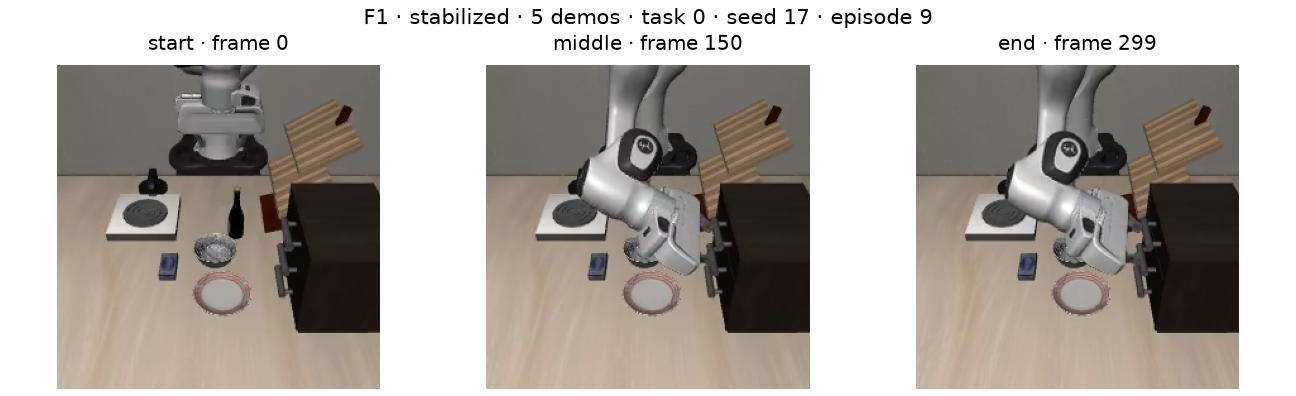
\includegraphics[width=\linewidth]{artifacts/results_v3/failures/failure-1.png}
\small\textbf{F1 / T0, 5 демо: контакт без открытия}
\end{minipage}\par\vspace{2pt}
\begin{minipage}[t]{\linewidth}\centering
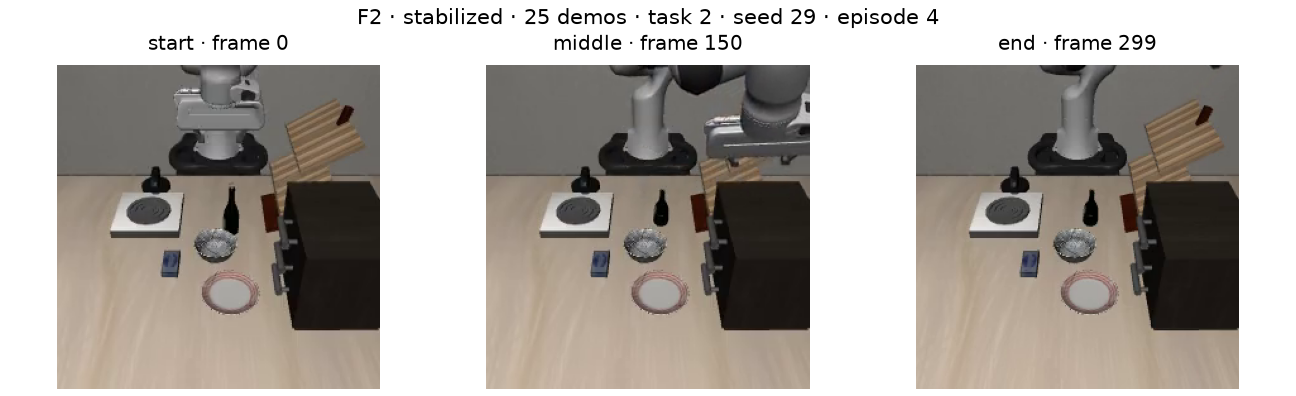
\includegraphics[width=\linewidth]{artifacts/results_v3/failures/failure-2.png}
\small\textbf{F2 / T2, 25 демо: отступление до захвата}
\end{minipage}\par\vspace{2pt}
\begin{minipage}[t]{\linewidth}\centering
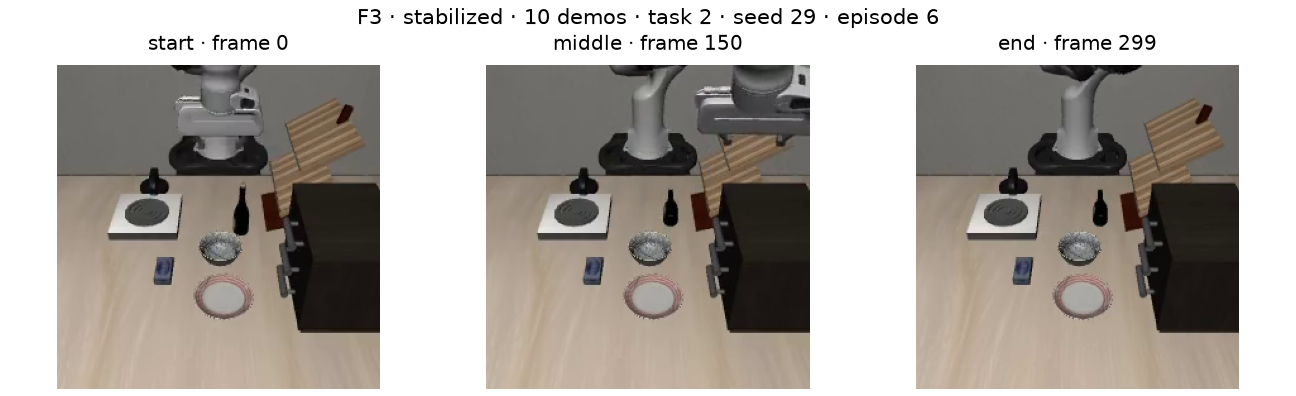
\includegraphics[width=\linewidth]{artifacts/results_v3/failures/failure-3.png}
\small\textbf{F3 / T2, 10 демо: повторная потеря цели}
\end{minipage}
\captionof{figure}{Детерминированно извлеченные кадры из трех фактических неуспешных CSWI rollout.
Это не демонстрации и не реконструкции; каждый эпизод содержит 300 кадров.}
\label{fig:failures}
\end{center}

Видео writer сохраняет меньше MP4, чем Boolean-исходов, поэтому три доступных failure cells покрывают
две задачи, а не искусственно создают пример T1. Количественные метрики всегда берутся из полного
\code{eval\_info.json}; video используется только для механистического анализа.

\section{Трассируемость примеров}

Каталог каждого кадра хранит stage, method, task, budget, training seed, список demo episode ID,
normalization scope, индекс evaluation episode, длину видео и исходный путь MP4. Селектор сначала
ищет неуспех для каждой задачи, затем добирает только новые task--budget--seed cells. Для T1
зарегистрированные неуспехи находятся за пределами первых MP4, сохраненных batched writer; поэтому
в отчет не подставлен успех, визуально похожий на отказ. Такая неполнота явно указана и не влияет на
Boolean-вектор метрики.

\newpage
\section{Механистические гипотезы}

\textbf{F1: контакт без открытия.} Эффектор достигает фасада у ручки, однако ящик не смещается.
Гипотеза --- неверное направление тяги после правильного grounding; альтернатива --- контакт с
ручкой не сформирован. Разделяющий тест логирует контакт, расстояние gripper--handle и силу вдоль оси
ящика. Устойчивый контакт без осевого смещения подтверждает control error; отсутствие контакта ---
grasp error.

\textbf{F2: раннее отступление.} Бутылка неподвижна, а рука уходит вверх и вправо до захвата.
Гипотеза --- первый reach не попадает в basin захвата; альтернатива --- action expert преждевременно
переключается на перенос. Oracle waypoint над бутылкой различит причины: восстановление захвата
указывает на perception/reach, повторный уход --- на ошибку фазы плана.

\textbf{F3: воспроизводимая потеря цели.} Независимая T2/$k=10$ ячейка повторяет тот же класс: объект
не сдвигается, эффектор покидает рабочую область. Следующий paired тест сравнивает minimum
EE--bottle distance и gripper phase у baseline, anchors и CSWI на одном reset state. Общий retreat
указывает на shared bias; исчезновение у одного anchor --- на destructive interpolation.

\section{Различающие эксперименты}

\begin{table}[h]
\centering\scriptsize
\begin{tabularx}{\linewidth}{@{}lXX@{}}\toprule
отказ & основное измерение & критерий различения\\\midrule
F1 & contact, axial force, handle distance & contact без смещения: control; нет contact: grasp\\
F2 & oracle waypoint над bottle & reach восстановлен: perception; retreat: plan phase\\
F3 & paired EE distance и gripper phase & общий retreat: shared bias; один anchor: interpolation\\
\bottomrule
\end{tabularx}
\tightcaption{Минимальные вмешательства, которые могут опровергнуть предложенный механизм.}
\end{table}

Ни один механизм не выводится только из финального кадра. Для каждого указана альтернативная причина,
наблюдаемая переменная и результат, меняющий интерпретацию. Это отделяет failure analysis от
постфактум описания движения.

Следующий прогон должен быть paired на уровне reset state и сравнить baseline, оба anchor и CSWI при
неизменных processor, action chunk и horizon. До запуска фиксируются три первичные переменные:
minimum object distance, первый устойчивый контакт и момент смены gripper phase. Проверка считается
разрешающей только тогда, когда заранее заданный паттерн отличает control, grasp, perception и
interpolation explanations; просмотр видео после метрики остается вспомогательным.

\clearpage

\section{Бонус B: video-only reward}

Малый action-free критик обучен только на seen-видео предсказывать нормированную временную позицию
кадра; action и simulator reward недоступны. Score --- среднее последних 10\% кадров. Robometer-4B
\cite{robometer} получает тот же детерминированный поднабор rollout и текст задачи. Эталон для аудита
--- simulator success по всем 20 эпизодам checkpoint cell.

\BonusText

\OptimizationText Это конечный zeroth-order optimizer над замороженным банком checkpoint, а не
gradient policy learning; его достоинство в том, что proxy выбирает policy до раскрытия полного
15-episode held-out simulator-аудита. Критики не влияли на выбор confirmatory checkpoint или CSWI.

\begin{table}[h]
\centering\small
\begin{tabular}{lrr}\toprule
критик & Spearman $\rho$ & span score\\\midrule
temporal critic & -0.323 & 0.0013\\
Robometer-4B & 0.252 & 0.298\\
\bottomrule
\end{tabular}
\tightcaption{Ранжирование 42 checkpoint cells против simulator success.}
\end{table}

\section{Воспроизводимость}

Четыре paired матрицы содержат 168 comparison-ячеек и 3,360 исходов; controls добавляют 480.
\code{vla-verify} проверяет пять preregistration, два protocol manifest, 192/192 ячейки,
длины Boolean-векторов, paired statistics, failure artifacts и Bonus B. Таблицы и векторный график
генерируются из CSV/JSON; сборка отклоняет любое число страниц, кроме четырех.

\section{Статистическая интерпретация}

Матрицы разных eval seed не пулируются: в них менялись и reset states, и заранее зарегистрированный
метод. Внутри фазы первично парное сравнение McNemar; Wilson CI описывает только абсолютную долю.
При 120 исходах на точку один эпизод равен 0.83 п.п., поэтому ranking около потолка дискретен и
неустойчив. После последовательной разработки не применяется постфактум multiple-testing claim:
Phase-II эффект рассматривается как hypothesis-generating, а v4/v5 --- как его опровержение.

\newpage

\section{Вывод и границы}

Первый общий вывод относится к интерфейсу: actuator contract является частью политики и должен
проверяться causal probe до дорогой матрицы. Второй относится к оптимизации: одинаковые данные не
делают один training seed свойством метода; комплементарность ошибок может быть
использована консервативным шагом в weight space.

\CeilingSummary\ \CeilingVerdict Независимые матрицы при этом меняют знак эффекта, поэтому общая
superior-claim принимается только если свежая ceiling-матрица проходит строгий критерий; иначе она
отвергается. Это не отсутствие результата:
показано, что при baseline 92--98\% 20 эпизодов на ветвь дают нестабильный ranking методов, а
weight-space regularization не гарантирует behavioral interpolation. Корректный следующий шаг ---
заранее фиксированный validation split, больше reset states и checkpoint averaging по траектории
обучения, а не следующий выбор маски на том же eval.

\section{Неожиданные наблюдения}

Синтаксически допустимое значение gripper не гарантировало физически корректного действия: один
потерянный знак полностью изменил success без исключения среды. Второе наблюдение: убедительный
single-seed cost-curve сдвиг исчез после смены reset states. Поэтому actuator probe, paired analysis
и независимый eval seed являются не отладочными деталями, а частью определения результата VLA.

\textbf{Ограничения.} Три задачи не представляют весь LIBERO-Goal; 20 эпизодов на ветвь дают широкие
интервалы; task prompts англоязычны; sparse success не измеряет качество частичного прогресса;
коэффициент смеси проверен только на данной архитектуре и conversion v3. Вывод не переносится
автоматически на absolute control, другие VLA или реальные роботы.

\begin{thebibliography}{3}\footnotesize
\bibitem{smolvla} M. Shukor et al. \emph{SmolVLA: A Vision-Language-Action Model for Affordable and
Efficient Robotics}. arXiv:2506.01844, 2025.
\bibitem{libero} B. Liu et al. \emph{LIBERO: Benchmarking Knowledge Transfer for Lifelong Robot
Learning}. NeurIPS Datasets and Benchmarks, 2023.
\bibitem{robometer} A. Liang et al. \emph{Robometer: Scaling General-Purpose Robotic Reward Models via
Trajectory Comparisons}. arXiv:2603.02115, 2026.
\end{thebibliography}

\end{document}
